%%
%  ******************************************************************************
%  * #file    Szablon_raportu_EN_Latex.tex
%  * #author  Adrian Wójcik   adrian.wojcik(at)put.poznan.pl
%  *          
%  * #commit  Patryk Kościk   koscikpatryk(at)gmail.com
%  *          Modified the template for Projekt przejsciowy purposes          
%  *          
%  * #version 1.0
%  * #date    09-Mar-2022
%  * #brief   PROJPRZEJ
%  *
%  ******************************************************************************
%%  
\documentclass[11pt, a4paper]{article}

\usepackage{Szablon_raportu_EN_Latex}

% Wypełnijcie te dyrektywy zgodnie z waszym tematem
% \lab      -> NAZWA CZUJNIKA, np.: 'DHT22'
% \comment  -> Króciutki opis co to, np.: 'Cyfrowy budżetowy czujnik temperatury'
%
\lab{GY-302}
\comment{moduł z czujnikiem oświetlenia BH1750}
\author{Hubert Pietrzak}

% Absolutny zakaz dotykania tego tutaj bo jak dotkiecie to coś jebnie
\university{Politechnika Poznańska}
\faculty{Wydział Automatyki, Robotyki i Elektrotechniki}
\institute{Instytut Robotyki i Inteligencji Maszynowej}
\department{Zakład Sterowania i Elektroniki Przemysłowej}
\addbibresource{Szablon_raportu_EN_Latex.bib}
\nocite{*}


%%
%
% Początek dokumentu
%
%%
\begin{document}

%% Strona tytułowa %%
\mainpage{BH1750}
\newpage

\section*{Opis elementu} \addcontentsline{toc}{section}{Wstęp}

GY-302 to moduł cyfrowego sensora oświetlenia z czujnikiem BH1750. Komunikacja z czujnikiem odbywa się poprzez wykorzystanie magistrali I2C. Ten układ scalony ma możliwe wykrywanie szerokiego zakresu  od 1 do 65535 lx z rozdzielczością 1 lub 4 lx w zależności od wyboru trybu pracy. Jasność jest konwertowana na sygnałc cyfrowy. Urządzenie ma niewielki pobór prądu ze względu na funkcję wyłączania. Dodatkowo układ ma funkcję filtrowania szumu przemysłowego w granicach 50-60 Hz. 


\vspace{0.5cm}
\begin{figure}[h]
\centering
\begin{subfigure}{.5\textwidth}
  \centering
  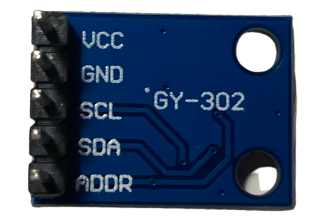
\includegraphics[width=.5\linewidth]{fig/obrazki/zdj_modułu/tyl-removebg-preview.png}
  \caption{tylnia część modułu i ich wyprowdzenia}
  \label{fig:sub1}
\end{subfigure}%
\begin{subfigure}{.5\textwidth}
  \centering
  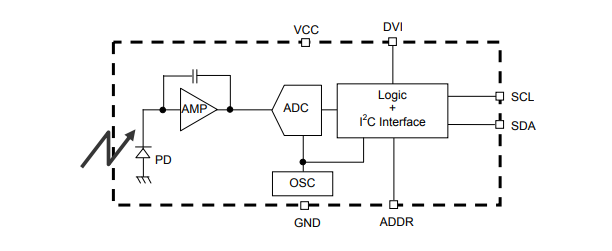
\includegraphics[width=.95\linewidth]{fig/obrazki/zdj_modułu/diagram.png}
  \caption{Diagram prezentujący działanie GY-302}
  \label{fig:sub2}
\end{subfigure}
\caption{Wyprowadzenia BH1750 i diagram działania komunikacji w czuniku}
\label{fig:test}
\end{figure}
\vspace{0.5cm}

%\subsection{Zasada działania}


BH1750 ma 5 wyprowadzeń pinów. Zasilanie \textbf{VCC} w zakresie od 3.3V do 5V i GND. Czujnik komunikuje się poprzez interfejs \textbf{I2C}, dzięki czemu mamy dwie linie danych- \textbf{SDA} - linia danych i \textbf{SCL} czyli linia zegara czasu rzeczwyistego.
Dodatkowo mamy wyprowadzenie \textbf{ADDR} służące do wyboru adresu magistrali I2C, podanie stanu niskiego ustala adres na: 0100011  wysokiego: 1011100. Domyślnie to wyprowadzenie znajduje się w stanie niskim.


\vspace{0.5cm}
\begin{figure}[h]
\centering
\begin{subfigure}{.5\textwidth}
  \centering
  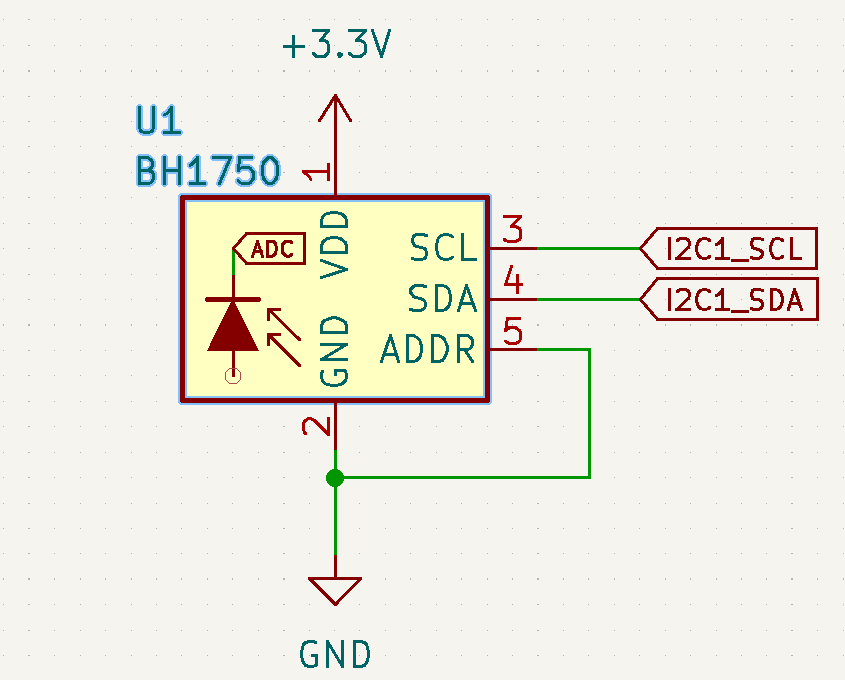
\includegraphics[width=.78\linewidth]{fig/obrazki/zasada_dzialania/BH.png}  
  \caption{Schemat elektryczny obwodu sensora cyfrowego BH1750}
  \label{fig:sub1}
\end{subfigure}%
\begin{subfigure}{.5\textwidth}
  \centering
  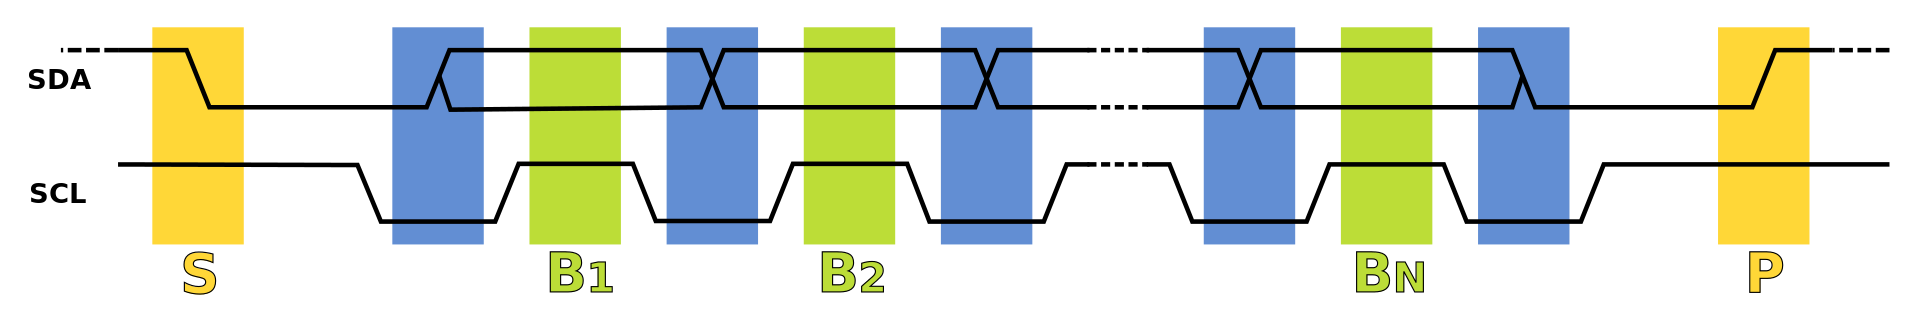
\includegraphics[width=.98\linewidth]{fig/obrazki/zasada_dzialania/I2C.png}
  \caption{Wzajemna praca zegara SCL i dostarczanych danych SDA}
  \label{fig:sub2}
\end{subfigure}
\caption{Schemat połączeń i praca danych i zegara czasu rzeczywistego}
\label{fig:test}
\end{figure}
\vspace{0.5cm}

%\subsection{Zastosowania}

Moduł GY-302 to specjalna płytka PCB, która zapewnia możliwość bezpośredniego podłączenia całego modułu do mikrokontrolera, bez wykorzystania prototywowych rezystorów typu pull-up/ pull-down czy wykorzystania kondensatorów filtrujących.


\begin{figure}[h!]
    \centering
    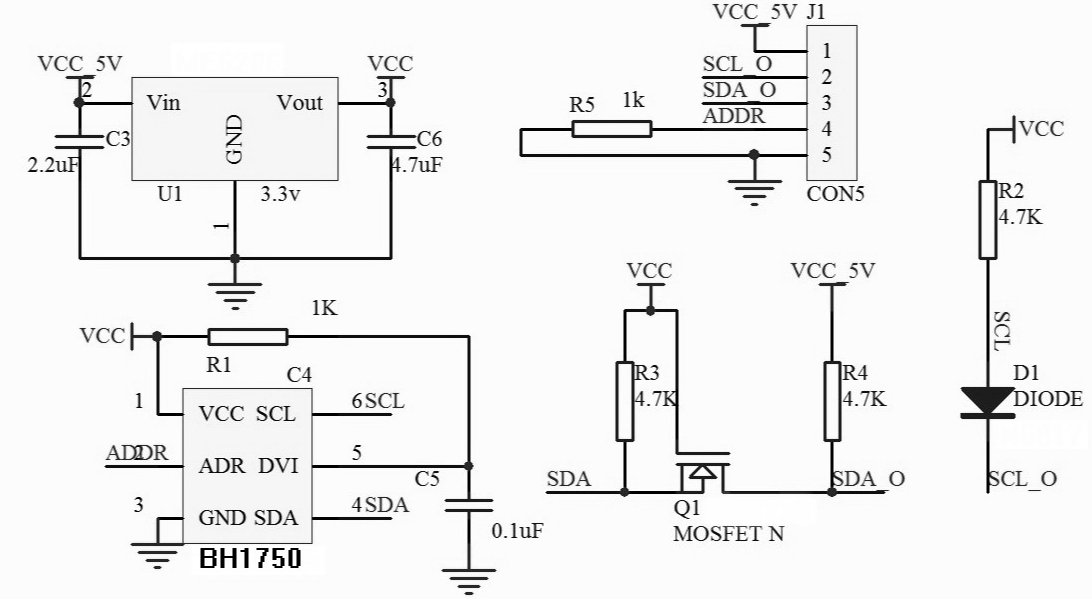
\includegraphics[width=0.8\textwidth]{fig/obrazki/działanie_ukladu/png_modified.png}
    \caption{Pełny schemat elektryczny modułu GY-302}
    \label{fig:my_label}
\end{figure}





\newpage

%\section{Implementacja czujnika}


% \vspace{0.5cm}

% \vspace{0.5cm}
% \begin{figure}[h!]
%     \centering
%     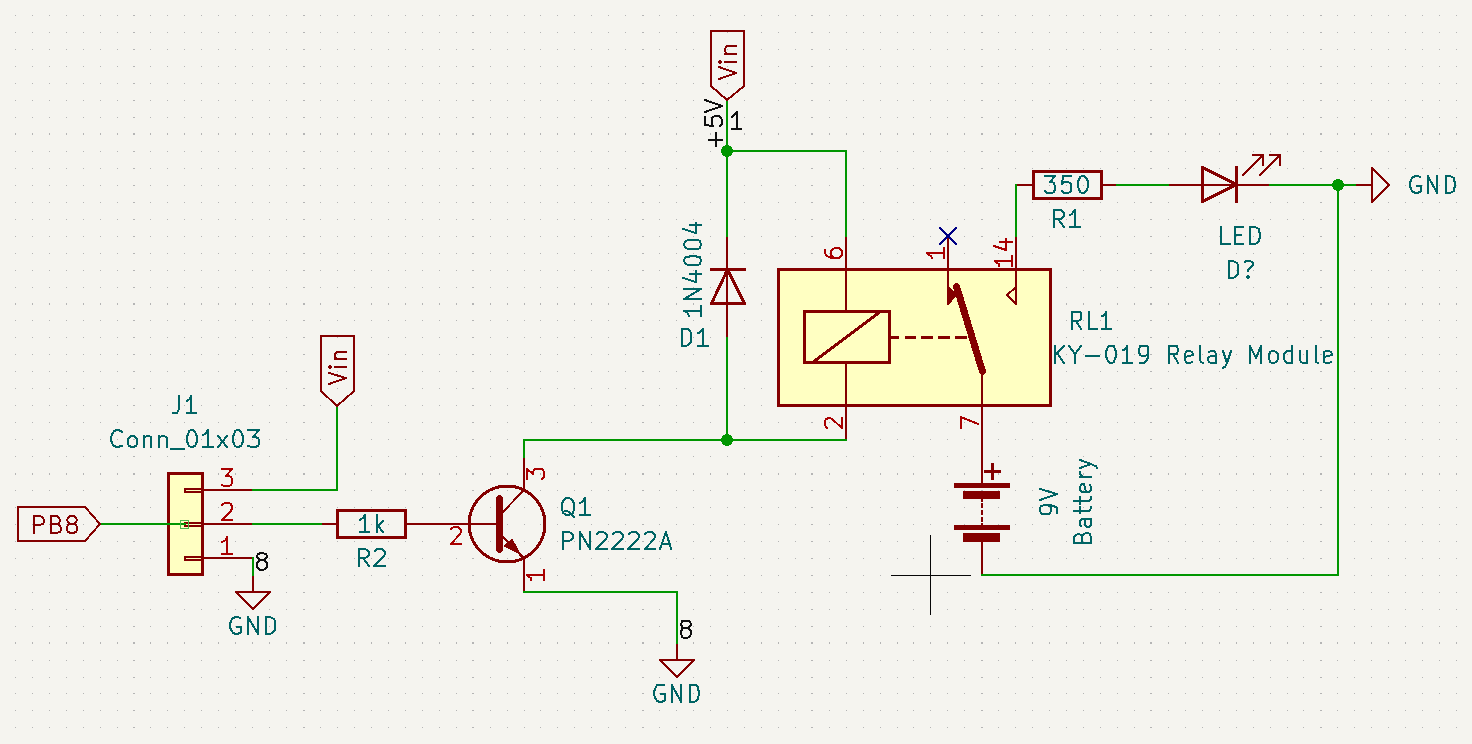
\includegraphics[scale=0.53]{fig/obrazki/polaczenie_modulu/Schematki.png}
%     \caption{Połaczenie elektryczne}
%     \label{fig:my_label}
% \end{figure}
% \vspace{0.5cm}


\newpage

%\section{Prezentacja działania układu}
\section{Użycie czujnika}



\vspace{0.5cm}
\begin{table}[h!]
    \centering
    \begin{tabular}{|c|c|c|c|} 
        \hline
        {NUCELO-F746ZG} & \multicolumn{2}{c|}{Moduł GY-320}  \\ 
        \hline
        Etykieta    &    Nr pinu &   Etykieta    \\ \hline
        +3V3    &        1   &   VCC \\  \hline
        GND     &      2   &   GND \\  \hline
        PB9     &      3   &   SCL \\  \hline
        PB6     &    4   &   SDA \\  \hline
        - & 5 & ADDR\\ \hline
    \end{tabular}
    \caption{Połącznie pomiędzy modułem i mikrokontrolerem}
    \label{tab:tab1}
\end{table}

% W określonych chwilach czasowych (tutaj przykładowo 1 sekunda) dzięki pinowi sterującemu, przekazujemy (lub też nie) sygnał na wyjście przekaźnika, co obserwujemy zmieniającym się stanem zmiennej \textbf{RelayState}

\begin{figure}[h!]
    \centering
    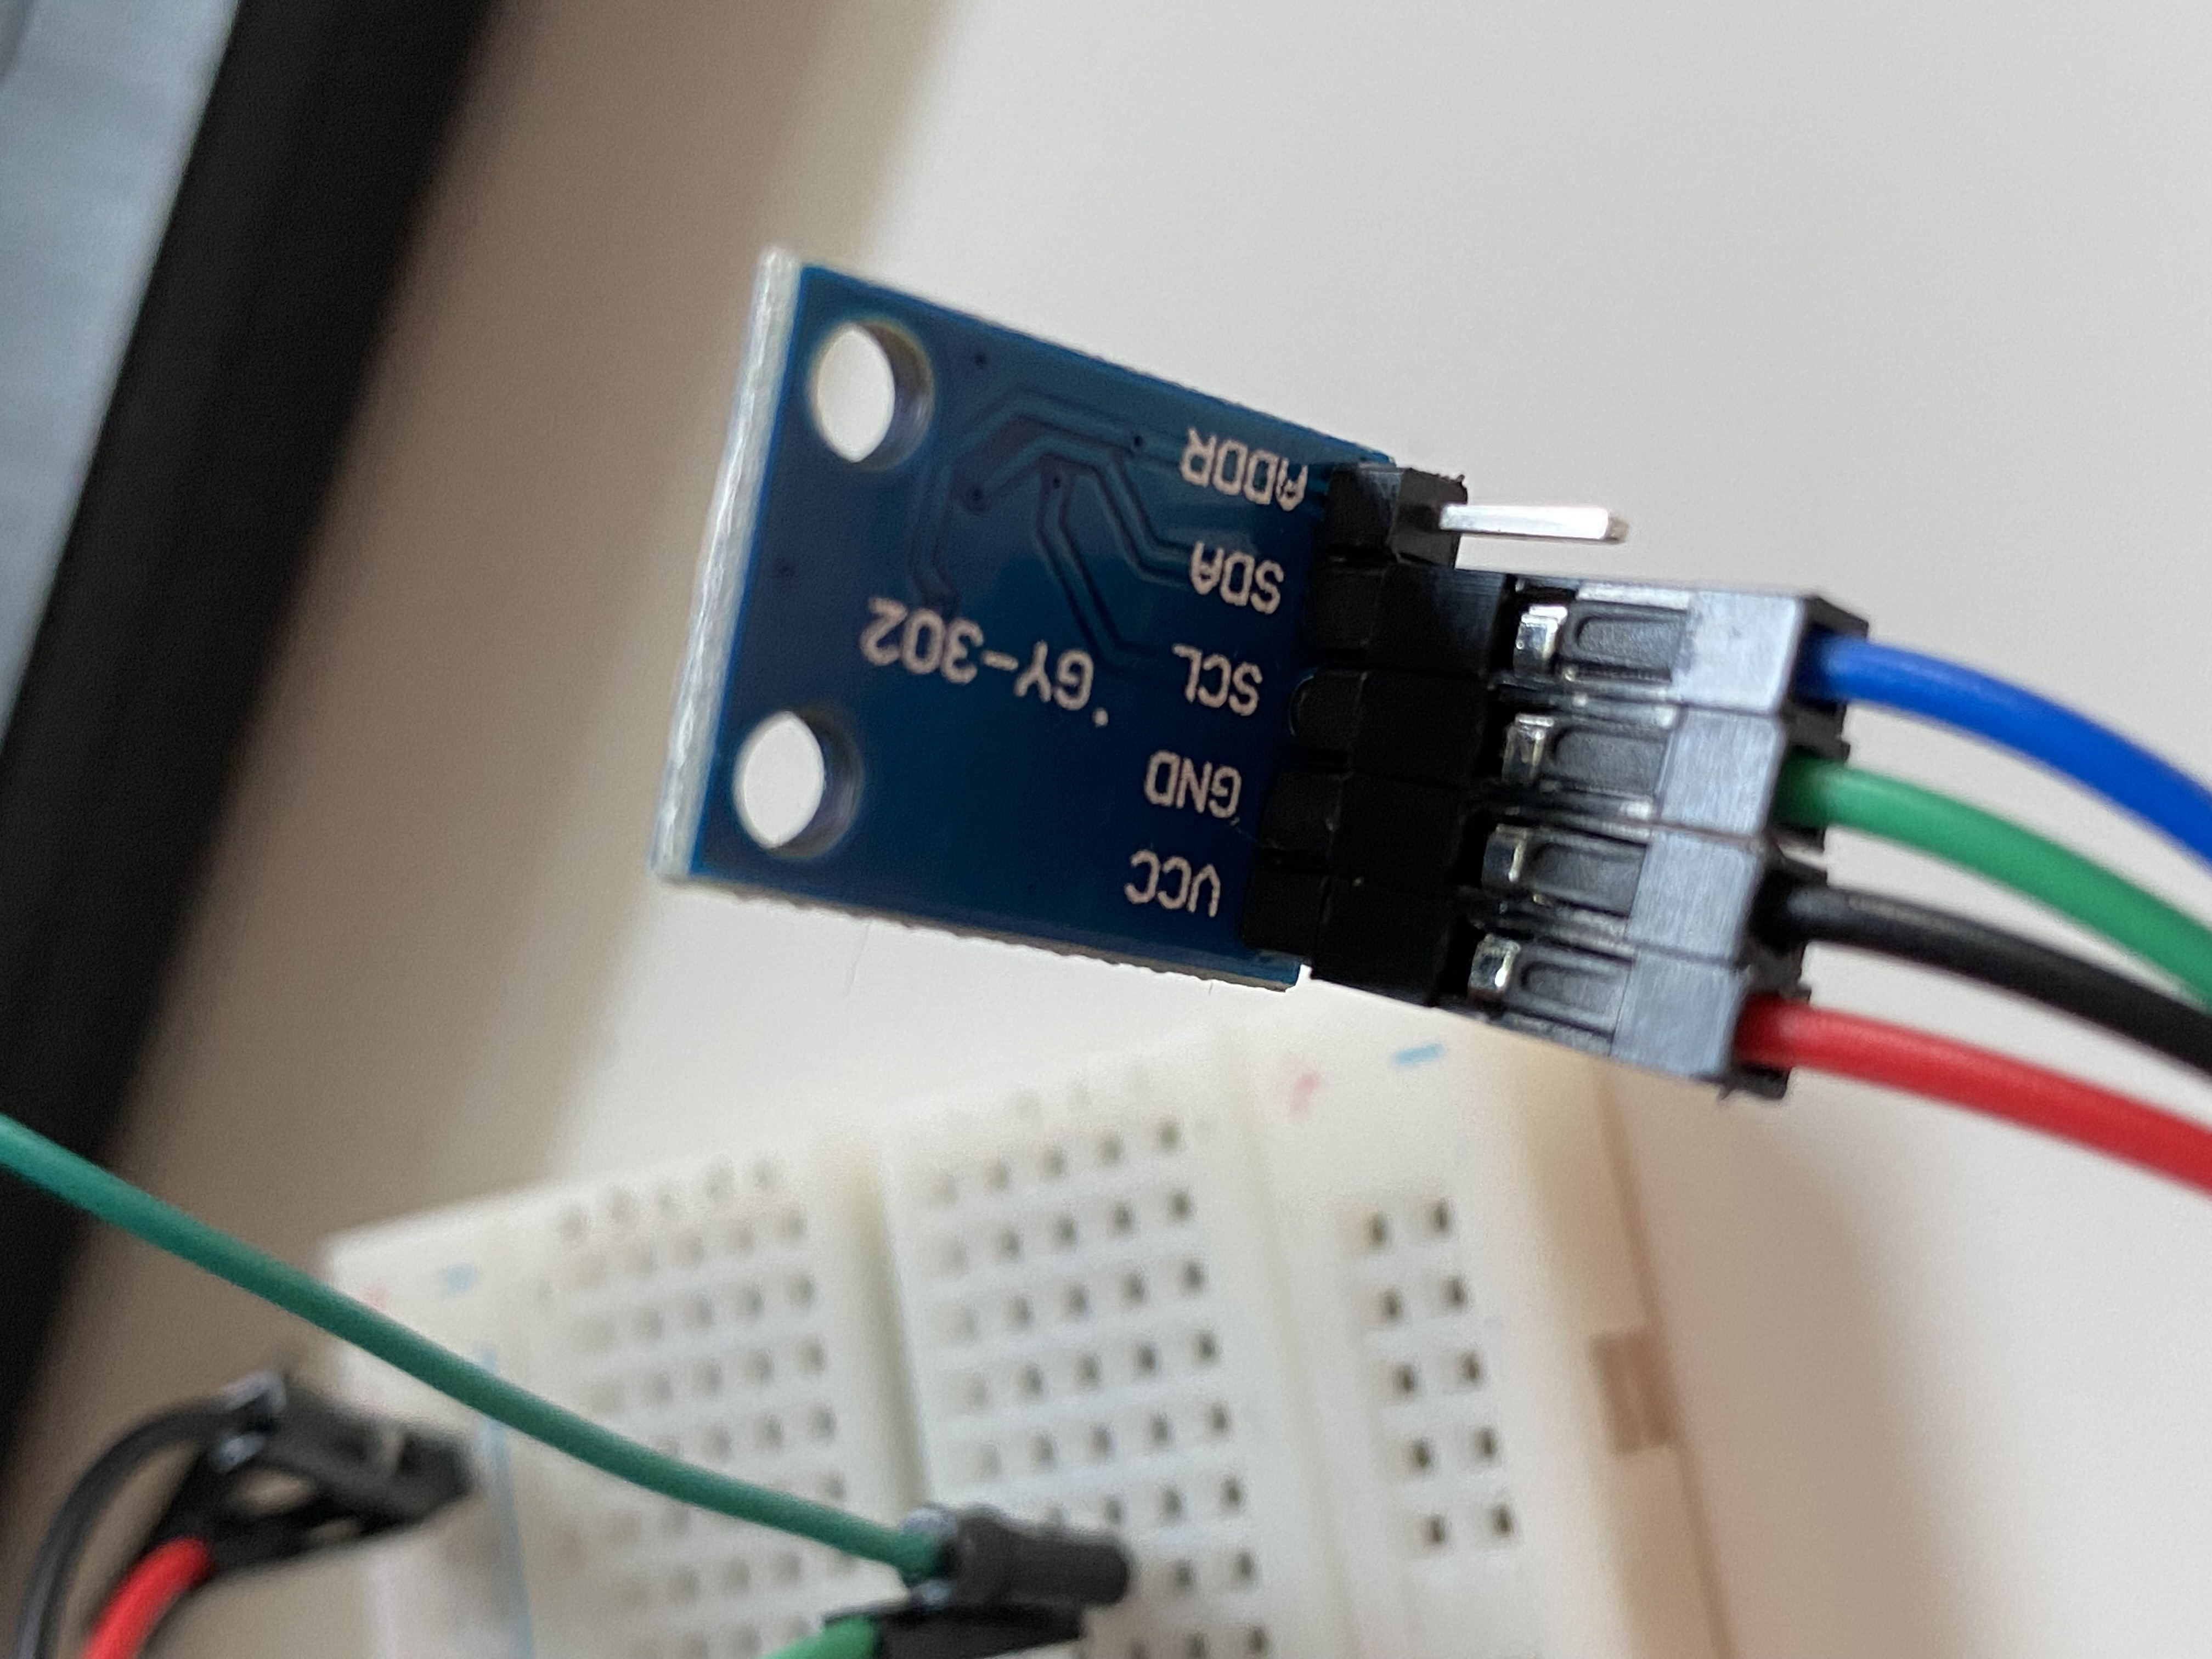
\includegraphics[scale=0.065]{fig/obrazki/działanie_ukladu/bh_nowy_obroot.jpg}
    \caption{podłaczenie wyprowadzeń pinowych}
    \label{fig:my_label}
\end{figure}

\vspace{0.5cm}
\begin{figure}[h!]
    \centering
    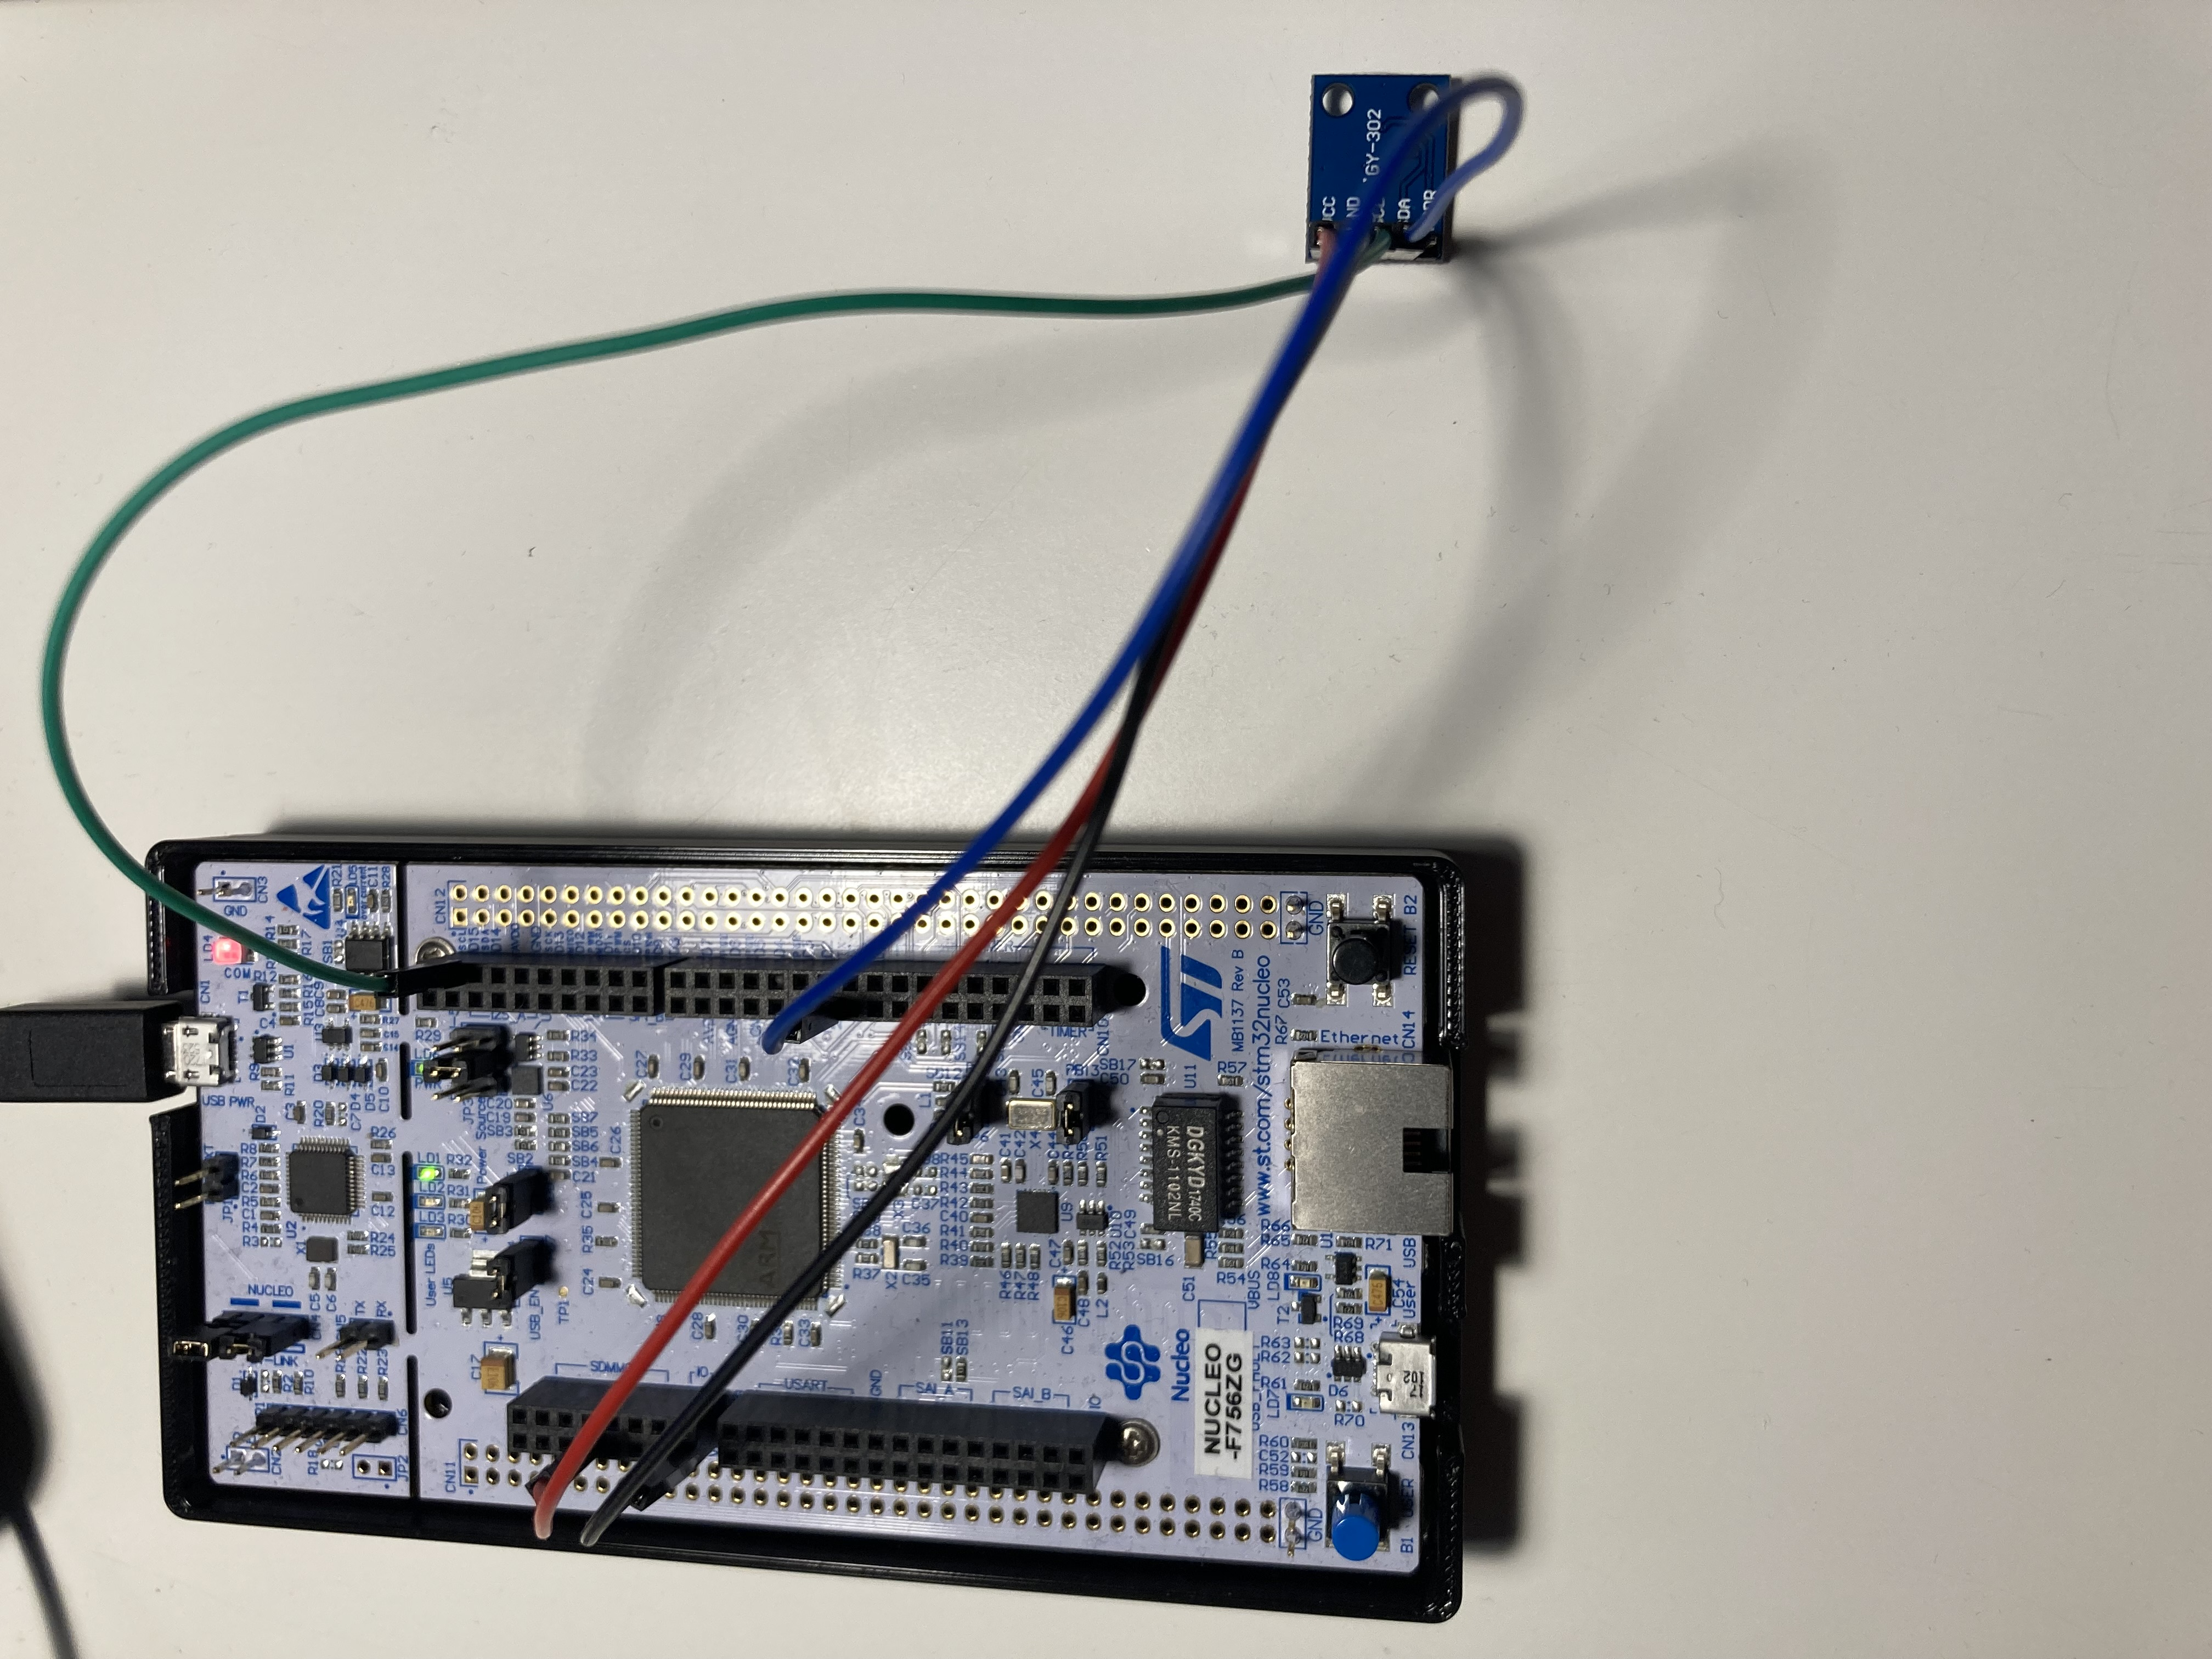
\includegraphics[scale=0.08]{fig/obrazki/działanie_ukladu/uklad.jpg}
    \caption{Rzeczywista realizacja układu}
    \label{fig:my_label}
\end{figure}
\vspace{0.5cm}

Działanie modułu w aplikacji z mikrokontrolerem zostało zaprezentowane na materiale wideo zawartym w % tu miejsce na odnosnik


% \vspace{0.5cm}
% \begin{figure}[h!]
%     \centering
%     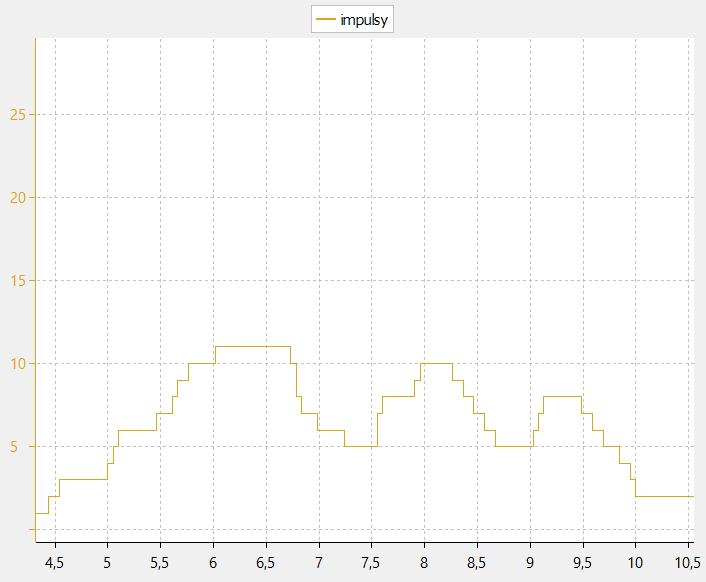
\includegraphics[scale=0.4]{fig/obrazki/działanie_ukladu/IMPULSY_PRZEBIEG.png}
%     \caption{Przebieg zmiany impulsów od czasu (obracanie enkoderem)}
%     \label{fig:my_label}
% \end{figure}
% \vspace{0.5cm}



\printbibliography[heading=bibintoc]

\end{document}